\documentclass[hidelinks,11pt,dvipsnames]{article}
% xcolor commonly causes option clashes, this fixes that
\PassOptionsToPackage{dvipsnames,table}{xcolor}
\usepackage[tmargin=1in, bmargin=1in, lmargin=0.8in, rmargin=1in]{geometry}

%%%%%%%%%%%%%%%%%%%%%%%%%%%%%%%%%%%%%%%%%%%%%%%%%%%%%%%%%%%%%%%%%%%%
%%% For inkscape-figures
%%% Assumes the following directory structure:
%%% master.tex
%%% figures/
%%%     figure1.pdf_tex
%%%     figure1.svg
%%%     figure1.pdf
%%%%%%%%%%%%%%%%%%%%%%%%%%%%%%%%%%%%%%%%%%%%%%%%%%%%%%%%%%%%%%%%%%%%
%\usepackage{import}
\usepackage{pdfpages}
\usepackage{transparent}

\newcommand{\incfig}[2][1]{%
    \def\svgwidth{#1\columnwidth}
    \import{./figures/}{#2.pdf_tex}
}

\pdfsuppresswarningpagegroup=1

% enable synctex for inverse search, whatever synctex is
\synctex=1
\usepackage{float,macrosabound,homework,theorem-env}
\usepackage{microtype}


% font stuff
\usepackage{sectsty}
\allsectionsfont{\sffamily}
\linespread{1.1}

% bibtex stuff
\usepackage[backend=biber,style=alphabetic,sorting=anyt]{biblatex}
\addbibresource{main.bib}

% colored text shortcuts
\newcommand{\blue}[1]{\color{MidnightBlue}{#1}}
\newcommand{\red}[1]{\textcolor{Mahogany}{#1}}
\newcommand{\green}[1]{\textcolor{ForestGreen}{#1}}


% use mathptmx pkg while using default mathcal font
\DeclareMathAlphabet{\mathcal}{OMS}{cmsy}{m}{n}

% fixes the positioning of subscripts in $$ $$
\renewcommand{\det}{\operatorname{det}}

\usetikzlibrary{positioning, arrows.meta}
\newcommand{\here}[2]{\tikz[remember picture]{\node[inner sep=0](#2){#1}}}

%%%%%%%%%%%%%%%%%%%%%%%%%%%%%%%%%%%%%%%%%%%%%%%%%%%%%%%%%%%%%%%%%%%%%
%%% Entry Counter
%%%%%%%%%%%%%%%%%%%%%%%%%%%%%%%%%%%%%%%%%%%%%%%%%%%%%%%%%%%%%%%%%%%%%
\newcounter{entry-counter}
\newcommand{\entry}[1]
{
	\addtocounter{entry-counter}{1}
    \tchap{Entry \arabic{entry-counter}}
	%\addcontentsline{toc}{section}{Entry \arabic{entry-counter}: #1}
	\vspace{-1.5em}
    \begin{center}
		\small \emph{Written: #1}
    \end{center}
}

\usepackage{titling}
\renewcommand\maketitlehooka{\null\mbox{}\vfill}
\renewcommand\maketitlehookd{\vfill\null}


\usepackage{capt-of}
\usepackage{tikz}
\usetikzlibrary{positioning,calc,intersections,through,backgrounds, shapes.geometric, decorations.markings,arrows}

\def\sset{\subseteq}
\def\iso{\cong}
\def\gend#1{\langle #1\rangle}

\newcommand{\rightoverleftarrow}{%
  \mathrel{\vcenter{\mathsurround0pt
    \ialign{##\crcr
      \noalign{\nointerlineskip}$\longrightarrow$\crcr
      \noalign{\nointerlineskip}$\longleftarrow$\crcr
    }%
  }}%
}

\newcommand\makesphere{} % just for safety
\def\makesphere(#1)(#2)[#3][#4]{%
  % Synopsis
  % \makesphere[draw options](center)(initial angle:final angle:radius)
  \shade[ball color = #3, opacity = #4] #1 circle (#2);
  \draw #1 circle (#2);
  \draw ($#1 - (#2, 0)$) arc (180:360:#2 and 3*#2/10);
  \draw[dashed] ($#1 + (#2, 0)$) arc (0:180:#2 and 3*#2/10);
}
% same thing as makesphere but places white background behind
\newcommand\altmakesphere{} % just for safety
\def\altmakesphere(#1)(#2)(#3)[#4][#5]{%
  % Synopsis
  % \make sphere[draw options](center)(initial angle:final angle:radius)
  \draw [fill=white!30] #1 circle (#2);
  \shade[ball color = #4, opacity = #5] #1 circle (#2);
  \draw #1 circle (#2);
  \draw ($#1 - (#2, 0)$) arc (180:360:#2 and 3*#2/10);
  \draw[dashed] ($#1 + (#2, 0)$) arc (0:180:#2 and 3*#2/10);
  \node at #1 {#3};
}

\begin{document}
% set section number to 1
% fixes theorem numbering without need to have a section title
\setcounter{section}{1}

\pagestyle{empty}
	\LARGE
\begin{center}
	Algebraic Topology Homework 13 \\
	\Large
	Isaac Martin \\
    Last compiled \today
\end{center}
\normalsize
\vspace{-4mm}
\hru

\tchap{Problems from 2.2}
\begin{homework}[e]
  \prob[\textsc{Exercise 15.}] Show that if $X$ is a CW complex then $H_n(X^n)$ is free by identifying it with the kernel of the cellular boundary map $H_n(X^n,X^{n-1})\to H_{n-1}(X^{n-1},X^{n-2})$.
  \begin{prf}
    This one seems so brief that I imagine I'm missing something or lacking justification. Essentially, this problem entails looking at the diagram on page 139 of Hatcher immediately preceding Theorem 2.35. It gives us an exact sequence
    \begin{align*}
      0 \to H_n(X^n) \xrightarrow{j_n} H_n(X^n,X^{n-1}) \xrightarrow{\partial_n} H_{n-1}(X^{n-1}).
    \end{align*}
    Since $j_n$ is injective, $H_n(X^n)$ is identified with $\img j_n = \ker \partial_n$. This alone should be enough to argue that $H_n(X^n)$ is injective, since $H_n(X^n,X^{n-1})$ is the free abelian group generated by the $n$-cells of $X$. However, as per the problem statement's instructions, we can also see this by identifying $X$ with the kernel of $d_n:H_n(X^n,X^{n-1})\to H_{n-1}(X^{n-1},X^{n-2})$, since $\ker d_n = \ker \partial_n$ by the injectivity of $j_n$. Here's a screencap of the diagram for reference:
    \begin{center}
      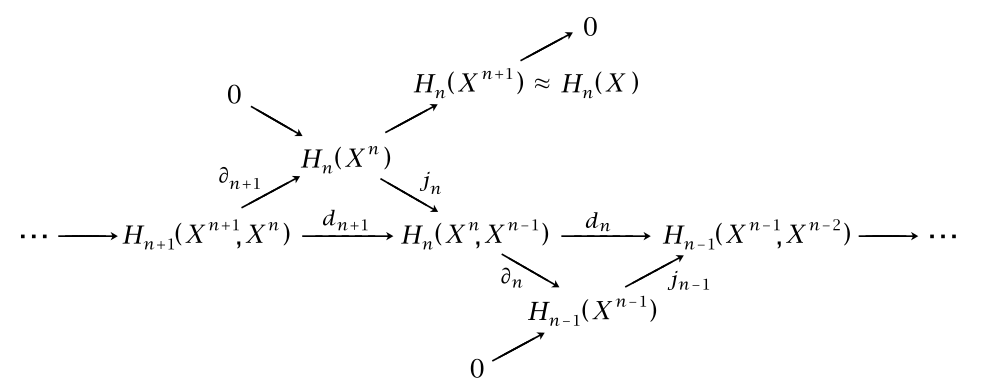
\includegraphics[width=12cm]{figures/hwk13-fig1.png}
      \captionof{figure}{Diagram on page 139 of Hatcher}
      \label{fig:prob15-1}
    \end{center}
  \end{prf}
  \prob[\textsc{Exercise 17.}] Show the isomorphism between cellular and singular homology is natural in the following sense: A map $f:X\to Y$ that is \emph{cellular} -- satisfying $f(X^n) \subseteq Y^n$ for all $n$ -- induces a chain map $f_*$ between the cellular chain complexes of $X$ and $Y$, and the map $f_*:H_n^{CW}(W) \to H_n^{CW}(Y)$ induced by this chain map corresponds to $f_*:H_n(X) \to H_n(Y)$ under the isomorphism $H_n^{CW}\approx H_n$.
  \begin{prf}
    Let $X$ and $Y$ be cell complexes and let $f:X\to Y$ be a cellular map so that $f(X^n) \subset Y^n$ for all $n$. The naturality of singular homology says that the diagram 
    \begin{center}  
    \begin{tikzcd}
        {H_n(X^n,X^{n-1})} & {H_{n-1}(X^{n-1})} & {H_{n-1}(X^{n-1},X^{n-2})} \\
        {H_n(Y^n,Y^n-1)} & {H_{n-1}(Y^{n-1})} & {H_{n-1}(Y^{n-1},Y^{n-2})}
        \arrow["{d_n}", curve={height=-24pt}, from=1-1, to=1-3]
        \arrow["{f_*}", from=1-1, to=2-1]
        \arrow["{f_*}", from=1-2, to=2-2]
        \arrow["{f_*}", from=1-3, to=2-3]
        \arrow["{d_n}", curve={height=24pt}, from=2-1, to=2-3]
    \end{tikzcd}
    \end{center}
    
    commutes, where $f_*$ is the map induced on singular homology. Thus, $f$ induces a cellular chain map $f_{\sharp}$ between the cellular chain complexes of $X$ and $Y$, that is, we have a commutative diagram
    \begin{center}
      \begin{tikzcd}
        ...\arrow[r]& H_n(X^{n+1},X^{n}) \arrow[d,"f_\sharp"] \arrow[r,"d_{n+1}"] & H_n(X^n,X^{n-1}) \arrow[d,"f_\sharp"] \arrow[r,"d_{n}"] & H_n(X^{n-1},X^{n-2}) \arrow[d,"f_\sharp"] \arrow[r] & ... \\
        ...\arrow[r]& H_n(Y^{n+1},Y^{n}) \arrow[r,"d_{n+1}"] & H_n(Y^n,Y^{n-1}) \arrow[r,"d_{n}"] & H_n(Y^{n-1},Y^{n-2}) \arrow[r] & ...
      \end{tikzcd}
    \end{center}
    This means $f$ induces a map on cellular homology, which we denote $f_*^{CW}$ in adherence to the problem's stated notation. Using the long exact sequence of the pair $(X^n,X^{n-1})$ along with Lemma 2.34, we get a commutative diagram
    \begin{center}
      \begin{tikzcd}
         &  &  &  0\arrow[d] & \\
        0 \arrow[r] & \img \partial_{n+1} \arrow[r]& H_n(X^n) \arrow[r,"i_n"]& H_n(X^n+1) \arrow[r]\arrow[d,"i_{n+1}"] & 0 \\
        &  &  &  H_n(X)\arrow[d] & \\
        &  &  &  0 & \\
      \end{tikzcd}
    \end{center}
    whose rows and columns are exact, where $i^n:X^n \to X^{n+1}$ is the inclusion map. Since $i_{n+1}i_{n}$ is the inclusion $X_n \hookrightarrow X$ we also have a short exact sequence
    \begin{align*}
      0 \to \img \partial_{n+1} \to H_n(X^n) \xrightarrow{i_n}H_n(X) \to 0.
    \end{align*}
  The proof of 2.35 (used for inspiration in problem 15 as well) tells us that the isomorphism $\varphi_X:H_n(X) \to H_n^{CW}(X)$ between singular and cellular homology is induced by $j_n$, i.e. it fits into the commutative diagram
  \begin{center}
    \begin{tikzcd}
      0 \arrow[r]& \img\partial_{n+1} \arrow[r]\arrow[d,"j_n"]& H_n(X^n) \arrow[r,"i_n"]\arrow[d,"j_n"] & H_n(X) \arrow[r] \arrow[d,"\varphi_X"]& 0 \\
      0 \arrow[r]& \img d_{n+1} \arrow[r]& \ker d_n \arrow[r]& H_n^{CW}(X) \arrow[r]& 0
    \end{tikzcd}
  \end{center}
  whose rows are exact. Imagine two copies of this diagram (I'm real tired of tikz), one for $X$ and one for $Y$, with corresponding entries in the top row connected via $f_*$ and entries in the bottom connected via $f_\sharp$. The top portion will commute by the naturality of singular homology, and by the isomorphism between singular and cellular homology the square
  \begin{center}
    \begin{tikzcd}
      H_n(X) \arrow[r,"f_*"] \arrow[d,"\varphi_X"] & H_n(Y) \arrow[d,"\varphi_Y"] \\
      H_n^{CW}(X) \arrow[r,"f_*^{CW}"] & H_n^{CW}(Y)
    \end{tikzcd}
  \end{center}
  commutes. This shows that the isomorphism between singular and cellular homology is indeed natural.
  \end{prf}
  \prob[\textsc{Exercise 19.}] Compute $H_i(\bRP^n/\bRP^m)$ for $m < n$ by cellular homology, using the standard CW structure on $\bRP^n$ with $\bRP^m$ as its $m$-skeleton.
  \begin{prf}
    Recall that the standard cell structure on $\bRP^n$ consists of a single $k$-cell for each $0\leq k\leq n$. The quotient $\bRP^n/\bRP^m$ amounts to collapsing all $k \leq m$ cells to a point, and thus yields us a cellular chain complex of the form
    \begin{align*}
      \bZ \xrightarrow{d_n} ... \xrightarrow{d_{m+2}} \bZ \xrightarrow{d_{m+1}} 0 \to ... \xrightarrow{d_1} \bZ \to 0,
    \end{align*}
    where $C^{CW}_k = 0$ for all $1 \leq k \leq m$ and is $\bZ$ for all other indices, including $d = 0$. The chain maps $d_k$ remain unchanged for $k > m$, i.e. we still have that
    \begin{align*}
      \ker(d_k) =
      \begin{cases}
        \bZ & k \text{ is odd } \\
        0 & k \text{ is even }
      \end{cases}
      \textbuff{2em}{and}
      \img(d_k) =
      \begin{cases}
        0 & k \text{ is odd } \\
        2\bZ & k \text{ is even }
      \end{cases},
    \end{align*}
    whereas $d_k$ is the trivial map for all $k \leq m$. Thus, working through the odd/even cases for both $m$ and $n$ gives us
    \begin{align*}
      H_k(\bRP^n/\bRP^m) =
      \begin{cases}
        \bZ & k = 0, ~k = m + 1 \text{ if $m$ is odd or} ~ k = n \text{ if $n$ is odd } \\
        \bZ_2 & k \text{ is odd and } m + 1 \leq k < n \\
        0 & \text{else}
      \end{cases}.
    \end{align*}
  \end{prf}
  \prob[\textsc{Exercise 20.}] For finite $CW$ complexes $X$ and $Y$, show that $\chi(X\times Y) = \chi(X)\chi(Y)$.
  \begin{prf}
    For a finite cell complex $X$, let $c_n(X)$ denote the number of $n$-cells. Let $X$ and $Y$ both be cell complexes. The $n$-cells in $X\times Y$ are simply the products of $i$-cells in $X$ and $j$-cells in $Y$ where $i + j = n$, as given in Appendix A.6 in Hatcher. But with this realization, we immediately have that
    \begin{align*}
      \chi(X\times Y) 
      &= \sum_{n} (-1)^{n} c_n(X\times Y) \\
      &= \sum_n \sum_{i+j = n}(-1)^{i+j}c_i(X)c_j(Y) \\
      &= \left(\sum_i (-1)^ic_i(X)\right) \left(\sum_{j}(-1)^j c_j(X)\right) \\
      &= \chi(X)\chi(Y),
    \end{align*}
    so we are actually done.
  \end{prf}
  \prob[\textsc{Exercise 21.}] If a finite CW complex $X$ is the union of subcomplexes $A$ and $B$, show that $\chi(X) = \chi(A) + \chi(B) - \chi(A\cap B)$.
  \begin{prf}
    This one is quick, as is the next one. As in question 20, let $c_n(X)$ denote the number of $n$-cells in a CW complex $X$. If $X$ is the union of two smaller subcomplexes, then $A\cap B$ is also a subcomplex of $X$ consisting of cells that are contained in both $A$ and $B$. We thus have that
    \begin{align*}
      c_n(X) = c_n(A) + c_n(B) - C_n(A\cap B),
    \end{align*}
    and hence
    \begin{align*}
      \chi(X) 
      &= \sum_n (-1)^{n} c_n(X) \\
      \sum_n(-1)^n(c_n(A) + c_n(B) - C_n(A\cap B)) \\
      &= \sum_n(-1)^nc_n(A)~+~\sum_n(-1)^nc_n(B)~-~\sum_n(-1)^nc_n(A\cap B) \\
      &= \chi(A) + \chi(B) - \chi(A\cap B).
    \end{align*}
  \end{prf}
  \prob[\textsc{Exercise 23.}] Show that if the closed orientable surface $M_g$ of genus $g$ is a covering space of $M_h$, then $g = n(h-1) + 1$ for some $n$, namely, $n$ is the number of sheets in the covering. [Conversely, if $g = n(h-1) + 1$] then there is an $n$-sheeted covering $M_g\to M_h$, as we saw in Example 1.41.]
  \begin{prf}
    Note that because $M_g$ is compact, any covering space $M_g\to M_h$ is finite sheeted. Consider such an $n$-sheeted covering space $M_g\to M_h$. We then have that
    \begin{align*}
      2 - 2g = \chi(M_g) = n\chi(M_h) = n(2 - 2h)
    \end{align*}
    by exercise 2.2.22, which says that $\chi(\tilX) = n\chi(X)$ when $p:\tilX\to X$ is an $n$-sheeted covering of finite cell complexes. Solving for $g$, we obtain the desired result $g = n(h - 1) + 1$.
  \end{prf}
  \prob[\textsc{Exercise 41.}] For $X$ a finite CW complex and $F$ a field, show that the Euler characteristic $\chi(X)$ can also be computed by the formula $\chi(X) = \sum_n(-1)^n \dim H_n(X;F)$, the alternating sum of the dimensions of the vector spaces $H_n(X;F)$.
  \begin{prf}
    Let $c_n$ denote the number of $n$-cells in $X$. Working over a field $F$ gives us a chain complex
    \begin{align*}
      ...\to F^{\oplus c_n} \xrightarrow{d_n} F^{\oplus c_{n-1}} \xrightarrow{d_{n-1}} ... \to F^{\oplus c_0} \to 0.
    \end{align*}
    Following the proof of Theorem 2.44, we have that $\dim F^{\oplus c_n} = c_n = \dim(\ker d_n) + \dim (\img d_{n})$ and $\dim(\ker d_n) = \dim(\img d_{n+1}) + \dim(H_n(X;F))$ by the rank-nullity theorem and the fact that $H_n(X;F) = \ker d_n/\img d_{n+1}$. Substituting the second equation into the first and multiplying by $(-1)^n$ gives us
    \begin{align*}
      (-1)^{n} c_n = (-1)^{n}\big(\dim(\img d_{n+1}) + \dim(H_n(X;F)) + \dim(\img d_n)\big),
    \end{align*}
    and summing over $n$ leads to cancellation of the $\dim(\img d_n)$ terms, yielding
    \begin{align*}
      \chi(X) = \sum_n(-1)^n c_n = \sum_n (-1)^n \dim H_n(X;F).
    \end{align*}
  \end{prf}
\end{homework}
\newpage
\tchap{Problems from 2.C}
\begin{homework}[e]
  \prob[\textsc{Exercise 2.}] Use the Lefschetz fixed point theorem to show that a map $S^n \to S^n$ has a fixed point unless its degree is equal to the degree of the antipodal map $x \mapsto -x$.
  \begin{prf}
    We first show that if $X$ is a path-connected simplicial complex then the map $f_*H_0(X)\to H_0(X)$ induced by a simplicial map $f:X\to X$ is the identity. The $0^{th}$ homology group is $H_0(X) = C_0(X)/\img(\partial_1) = \bZ$ by path-connectedness, so all vertices lie in the same homology class. Since $f_*$ is simplicial, we thus have that $f_*([v]) = [f(v)] = [v]$ for any vertex $v$ of $X$, hence $f_*$ is the identity. By simplicial approximation, it follows that any continuous map $f:X\to X$ is homotopic to a simplicial map as long as $X$ is a finite simplicial complex, after barycentric subdividing if necessary, at least. Hence, any map $f:X\to X$ in this setup satisfies $\tr(f_*) = 1.$ In particular, this holds when $X = S^n$.

    Now we calculate the Lefschetz number for a map $f:S^n \to S^n$:
    \begin{align*}
      \tau(f)
      &= \sum_i (-1)^i \tr(f_*:H_i(S^n) \to H_i(S^n)) \\
      &= \tr(f_*:H_0(S^n) \to H_0(S^n)) + (-1)^n \tr(f_*:H_n(S^n)\to H_n(S^n)) \\
      &= 1 + (-1)^n\tr(f_*:H_n(S^n) \to H_n(S^n))
    \end{align*}
    because $H_i(S^n) = 0$ unless $i = 0,n$. By the Lefschetz fixed point theorem, there exists some fixed point whenever $\tau(f) \neq 0$. We see that $\tau(f) = 0$ if and only if $\deg(f) = (-1)^{n+1}$; that is, if $f$ has the same degree as the antipodal map.
  \end{prf}
  \prob[\textsc{Exercise 4.}] This one was just too long, I couldn't finish it in time.
  \prob[\textsc{Exercise 5.}] Let $M$ be a closed orientable surface embedding in $\bR^3$ in such a way that reflection across a plane $P$ defines a homeomorphism $r:M\to M$ fixing $M\cap P$, a collection of circles. Is it possible to homotope $r$ to have no fixed points?
  \begin{prf}
    First consider a homeomorphism $h:S^1\times I \to S^1\times I$, where
    \begin{align*}
      (e^{i\theta},\alpha)\mapsto
      \begin{cases}
        (e^i\theta + 2\pi \alpha,\alpha) & \alpha \in [0,1/2] \\
        (e^{i\theta + 2\pi(1 - \alpha)}, \alpha) & \alpha \in (1/2,1]
      \end{cases},
    \end{align*}
    i.e. as $\alpha$ moves from $0$ to $1/2$ the circle attached to $\alpha$ is rotated an increasing amount until we reach $\alpha = 1/2$, at which point the circles rotate back to the original position. This map fixes the boundary of $S^1\times I$, since $S^1\times \{0,1\}$ experiences no rotation.
    \begin{center}
      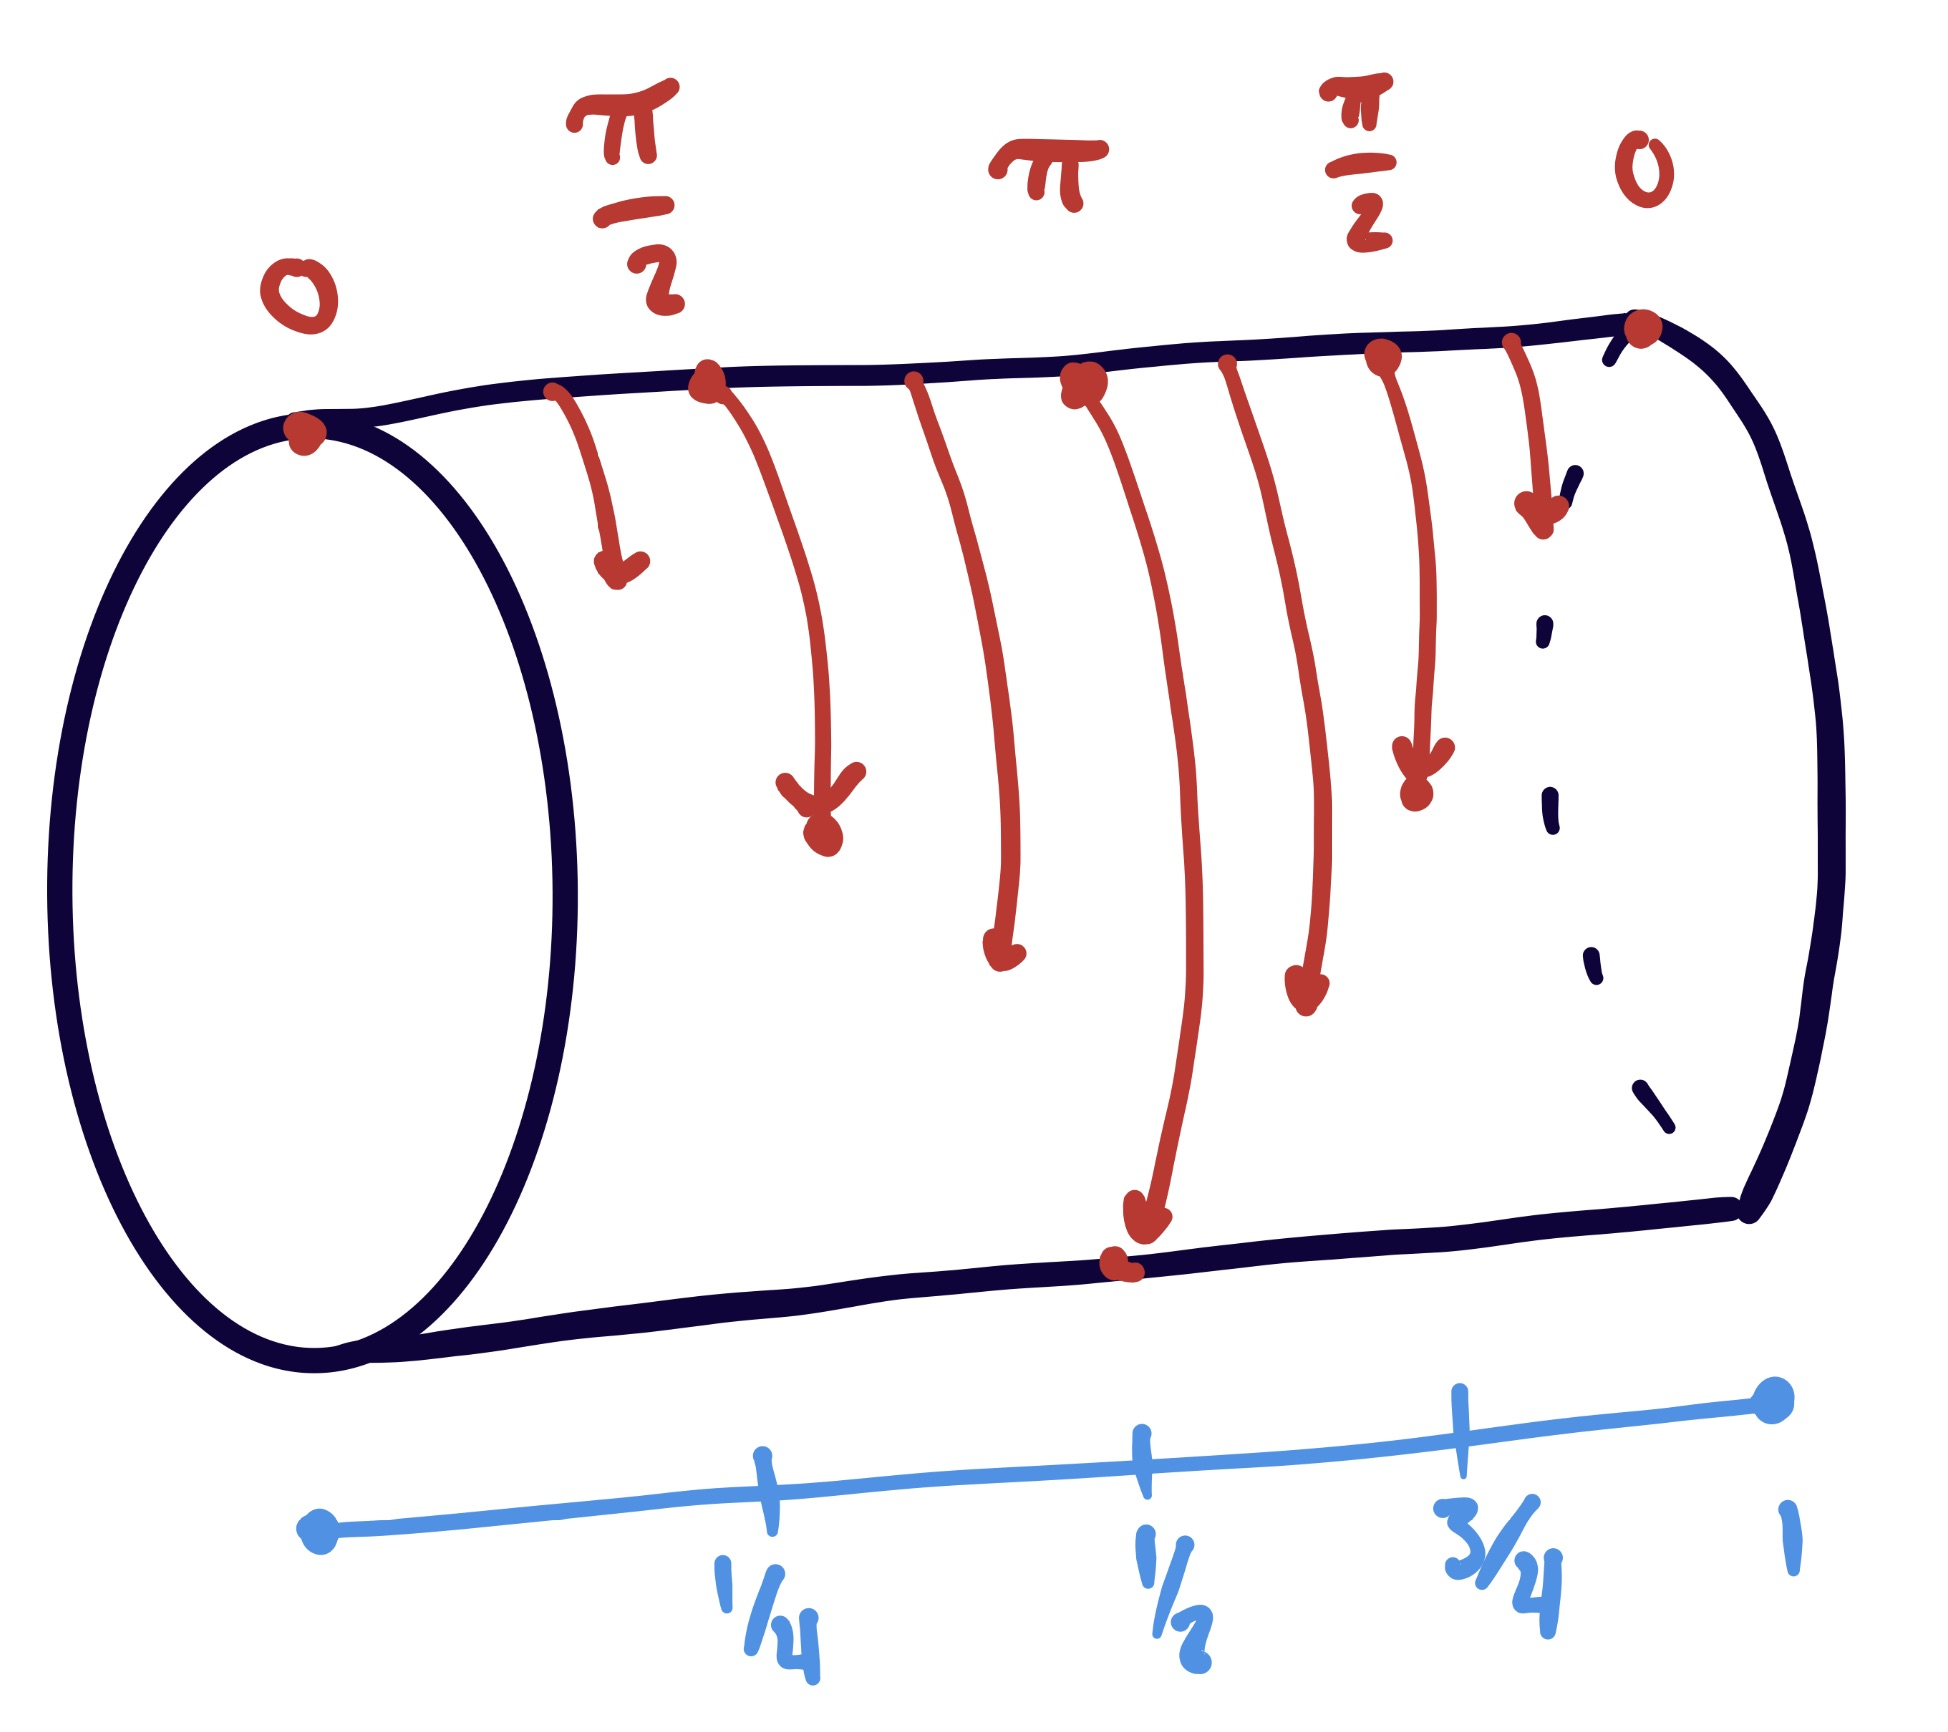
\includegraphics[width=9cm]{figures/hwk13-fig2.png}
      \captionof{figure}{Illustration of the homeomorphism $h$ on the cylinder}
      \label{fig:prob15-2}
    \end{center}
    Note that $h$ is homotopic to the identity on $S^1\times I$, since we can simply interpolate each angle of rotation at a constant rate to 0. 

    For each circle in $M\cap P$, consider a band $N \cong S^1 \times I$ contained in $M$ such that $M\cap P$ is identified with $S^1 \times \{1/2\}$ and apply the homeomorphism $h$. Crucially, no points of $M\cap P$ are fixed by $h$. Doing this for each circle and extending by the identity on $M \setminus P$ yields a homeomorphism $\olh:M\to M$, which is homotopic to the identity via the same homotopy yielding $h \simeq \id_{S^1\times I}$ by extending by the identity outside of $M\cap P$. Thus, $r\circ \olh \simeq r\circ \id_M$ and has no fixed points.
  \end{prf}
\end{homework} 
\end{document}
